\documentclass[11pt,a4paper]{article}
\usepackage[utf8]{inputenc}
\usepackage[T1]{fontenc}
\usepackage{lmodern}
\usepackage[margin=2cm]{geometry}
\usepackage{amsmath}
\usepackage{booktabs}
\usepackage{xcolor}
\usepackage{enumitem}
\usepackage{pgfplots}
\usepgfplotslibrary{groupplots}
\pgfplotsset{compat=1.18}
\usepackage[font=small,labelfont=bf,skip=4pt]{caption}
\usepackage[hidelinks]{hyperref}

\definecolor{yblue}{HTML}{2A78D6}
\definecolor{yorange}{HTML}{EB6834}
\definecolor{yaqua}{HTML}{1BAF7A}

\setlist{itemsep=2pt, topsep=3pt}
\setlength{\textfloatsep}{10pt}

\newcommand{\myname}{Marius Casamian}

\begin{document}

\begin{center}
  {\Large\bfseries Monitoring the YEGO scooter fleet in Nice with public GBFS data}\\[4pt]
  \myname\ --- application for the Data Analyst -- Operations position (V.I.E.\ 246717)\\
  24 October 2026 \quad $\cdot$ \quad Code and data: \url{https://github.com/MariusEtudiant/yego-nice-ops}
\end{center}

\begin{abstract}
\noindent YEGO publishes the position and battery level of its scooters in real time through the
General Bikeshare Feed Specification (GBFS). I collected this feed every two minutes in Nice and
Barcelona from Sunday 11 October at 18:23 to Saturday 24 October at 10:47 (8,308 snapshots for Nice, including 10
complete days) and computed operational indicators with dbt. Three findings stand out for Nice:
(i) on 9 of the 10 evenings observed, most battery swaps came after the demand peak,
while about 27 scooters were waiting for a battery at that peak; (ii) a scooter disabled
for low battery waits 5.3\,h (median) before its swap, about twice as long as in Barcelona;
(iii) 12.6\% of the fleet is disabled for reasons other than battery, often for days.
\end{abstract}

\section{Data and method}

\textbf{Data.} For every scooter that is parked and not rented, the feed \cite{gbfs} gives its
position, battery level and two flags, \texttt{is\_reserved} and \texttt{is\_disabled}. A Python
collector, first on my computer and then on GitHub Actions every hour, stores each snapshot as a
Parquet file. The collection has one interruption of 35\,h (12--13 October) and is complete
from Wednesday 14 October to Friday 23 October; daily averages below use only these 10 complete days.

\textbf{Anonymised identifiers.} The \texttt{bike\_id} field is regenerated at every request, so a
scooter cannot be followed through its identifier. I match the scooters of two consecutive snapshots:
a pair $(i,j)$ is a candidate if both have the same type and are less than 15\,m apart, with cost
\begin{equation}
  c_{ij} = d_{ij} + \lambda\,\lvert b_i - b_j \rvert, \qquad \lambda = 0.5\ \text{m per battery point},
\end{equation}
where $d_{ij}$ is the distance and $b$ the battery level. I keep the one-to-one matching with the
lowest total cost (Hungarian algorithm \cite{kuhn1955}), plus a second pass for GPS jumps up to
150\,m when the battery is unchanged. 99.6\% of the observations are linked to a scooter of
the previous snapshot.

\textbf{Events and quality checks.} A \emph{departure} is a scooter that disappears from the feed
(rented, or picked up by the staff). A \emph{battery swap} is a rise of at least 20 battery points on
the same scooter. A \emph{battery wait} runs from the moment a scooter is disabled for low battery
to the moment it leaves this state. Everything is modelled with dbt on DuckDB \cite{duckdb}, with
data tests on keys, relationships, positions, collection gaps and business rules
(33 passed, 4 warnings, 0 failed). The warnings are real findings, described in Section~\ref{sec:quality}.

\section{Results}

\textbf{Fleet availability.} On average 235 scooters were listed in Nice and 75\%
were available (Figure~\ref{fig:fleet}). 10.8\% were disabled because of their battery and
12.6\% for another reason. No active scooter had less than 15\% battery, apart from a few
transient cases in Barcelona, so YEGO disables scooters under this threshold. The battery queue
never empties: between 23 and 31 scooters are waiting at any hour of an average day.
In Barcelona, 86\% of the scooters are available and only 4.3\% wait for
a battery. Nice has about 3.1 departures per scooter and per day (725 in
total).


\begin{figure}[ht]
  \centering
  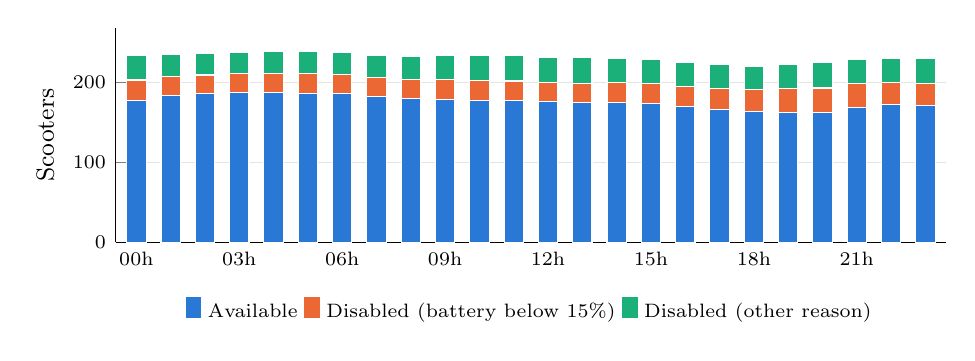
\begin{tikzpicture}
    \begin{axis}[
        ybar stacked, bar width=7pt, width=\linewidth, height=4.3cm,
        ymin=0, ymax=268, xmin=-0.6, xmax=23.6,
        xtick={0,...,23}, xticklabels={00h,,,03h,,,06h,,,09h,,,12h,,,15h,,,18h,,,21h,,},
        tick label style={font=\scriptsize}, ylabel={Scooters},
        ylabel style={font=\small}, axis x line*=bottom, axis y line*=left,
        ymajorgrids, grid style={black!10},
        legend style={at={(0.5,-0.22)}, anchor=north, legend columns=3, draw=none, font=\scriptsize},
        legend cell align=left]
      \addplot[fill=yblue, draw=white] coordinates {(0,177.37) (1,184.13) (2,186.35) (3,187.54) (4,187.88) (5,186.15) (6,185.80) (7,183.04) (8,180.10) (9,178.62) (10,177.75) (11,178.04) (12,176.12) (13,175.39) (14,175.42) (15,173.67) (16,169.86) (17,166.48) (18,163.39) (19,162.77) (20,162.28) (21,168.97) (22,172.06) (23,171.20)};
      \addplot[fill=yorange, draw=white] coordinates {(0,25.75) (1,22.93) (2,23.02) (3,23.62) (4,23.99) (5,24.70) (6,24.12) (7,23.54) (8,23.90) (9,24.65) (10,24.34) (11,23.89) (12,23.66) (13,23.91) (14,24.13) (15,24.78) (16,25.46) (17,26.17) (18,27.98) (19,29.54) (20,30.90) (21,29.35) (22,28.17) (23,28.06)};
      \addplot[fill=yaqua, draw=white] coordinates {(0,30.95) (1,28.63) (2,27.24) (3,26.84) (4,27.05) (5,28.04) (6,27.87) (7,27.79) (8,28.62) (9,30.28) (10,31.95) (11,31.46) (12,31.94) (13,31.52) (14,31.04) (15,30.56) (16,29.94) (17,29.63) (18,29.36) (19,30.17) (20,31.42) (21,30.09) (22,29.63) (23,31.07)};
      \legend{Available, Disabled (battery below 15\%), Disabled (other reason)}
    \end{axis}
  \end{tikzpicture}
  \caption{Scooters listed in the Nice feed by hour of the day, mean over 10 complete days.
  Reserved scooters are not shown; rented scooters are not in the feed.}
  \label{fig:fleet}
\end{figure}


\textbf{Battery swaps and demand.} I detected 71 battery swaps per day in Nice;
90\% of them on a disabled scooter, whose battery went from 17\% to
88\% on average. Demand peaks at the end of the afternoon, and every evening the busiest
hour was 17h or 18h (Table~\ref{tab:evenings}). Swaps, however, are concentrated between 20h and
2h (Figure~\ref{fig:timing}): on average 66\% of the swaps of an evening and night
came after its peak (from 42\% to 81\% depending on the evening). The queue is
also not emptied by the morning: 10 to 44 scooters were still waiting
between 5h and 9h.


\begin{figure}[ht]
  \centering
  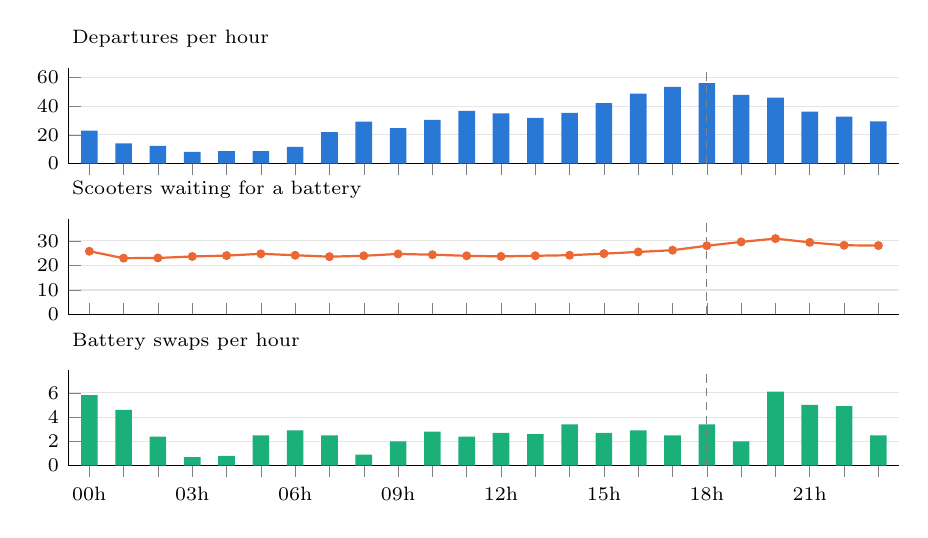
\begin{tikzpicture}
    \begin{groupplot}[
        group style={group size=1 by 3, vertical sep=0.7cm, xticklabels at=edge bottom},
        title style={font=\scriptsize, at={(0,1)}, anchor=south west, inner sep=1pt},
        width=\linewidth, height=2.8cm, xmin=-0.6, xmax=23.6,
        xtick={0,...,23}, xticklabels={00h,,,03h,,,06h,,,09h,,,12h,,,15h,,,18h,,,21h,,}, ymin=0,
        tick label style={font=\scriptsize},
        axis x line*=bottom, axis y line*=left, ymajorgrids, grid style={black!10}]
      \nextgroupplot[ybar, bar width=6pt, ymax=67, title={Departures per hour}]
        \addplot[fill=yblue, draw=none] coordinates {(0,22.90) (1,14.10) (2,12.30) (3,8.10) (4,8.60) (5,8.60) (6,11.70) (7,21.90) (8,29.20) (9,24.70) (10,30.40) (11,36.80) (12,35.10) (13,31.80) (14,35.30) (15,42.20) (16,48.80) (17,53.60) (18,56.10) (19,48.00) (20,46.10) (21,36.20) (22,32.70) (23,29.50)};
        \draw[densely dashed, black!50] (axis cs:18,0) -- (axis cs:18,67.3);
      \nextgroupplot[ymax=39, title={Scooters waiting for a battery}]
        \addplot[yorange, thick, mark=*, mark size=1.2pt] coordinates {(0,25.75) (1,22.93) (2,23.02) (3,23.62) (4,23.99) (5,24.70) (6,24.12) (7,23.54) (8,23.90) (9,24.65) (10,24.34) (11,23.89) (12,23.66) (13,23.91) (14,24.13) (15,24.78) (16,25.46) (17,26.17) (18,27.98) (19,29.54) (20,30.90) (21,29.35) (22,28.17) (23,28.06)};
        \draw[densely dashed, black!50] (axis cs:18,0) -- (axis cs:18,38.6);
      \nextgroupplot[ybar, bar width=6pt, ymax=7.9, title={Battery swaps per hour}]
        \addplot[fill=yaqua, draw=none] coordinates {(0,5.80) (1,4.60) (2,2.40) (3,0.70) (4,0.80) (5,2.50) (6,2.90) (7,2.50) (8,0.90) (9,2.00) (10,2.80) (11,2.40) (12,2.70) (13,2.60) (14,3.40) (15,2.70) (16,2.90) (17,2.50) (18,3.40) (19,2.00) (20,6.10) (21,5.00) (22,4.90) (23,2.50)};
        \draw[densely dashed, black!50] (axis cs:18,0) -- (axis cs:18,7.9);
    \end{groupplot}
  \end{tikzpicture}
  \caption{Demand, battery queue and battery swaps in Nice by hour of the day, mean over
  10 complete days. The dashed line marks the busiest hour.}
  \label{fig:timing}
\end{figure}



\begin{table}[ht]
  \centering
  \small
  \begin{tabular}{lrrrrr}
    \toprule
    Evening & Busiest hour & Departures & Waiting for & Battery swaps & Swaps done \\
            & (16h--22h)   & that hour  & a battery   & (until 10h)   & after the peak \\
    \midrule
    Wed 14/10 & 18h & 65 & 27 & 68 & 63\% \\
    Thu 15/10 & 17h & 63 & 49 & 77 & 75\% \\
    Fri 16/10 & 17h & 66 & 31 & 81 & 69\% \\
    Sat 17/10 & 18h & 80 & 34 & 93 & 81\% \\
    Sun 18/10 & 18h & 39 & 34 & 81 & 77\% \\
    Mon 19/10 & 17h & 66 & 27 & 64 & 58\% \\
    Tue 20/10 & 18h & 49 & 12 & 59 & 42\% \\
    Wed 21/10 & 18h & 55 & 15 & 56 & 54\% \\
    Thu 22/10 & 17h & 54 & 19 & 60 & 73\% \\
    Fri 23/10 & 18h & 61 & 25 & 84 & 63\% \\
    \bottomrule
  \end{tabular}
  \caption{Evening by evening in Nice: the busiest hour, the scooters waiting for a battery at
  that hour, and the share of the following battery swaps that came after it.}
  \label{tab:evenings}
\end{table}


\textbf{Battery waiting time.} Once disabled for low battery, a scooter in Nice waits
5.3\,h before its swap (median); a quarter wait more than 12.1\,h and a tenth more than
22.7\,h. In Barcelona the median is only 2.6\,h (a quarter wait more than 5.5\,h). The hour matters: scooters disabled between 11h and
16h wait 7.0\,h (median), because they are only handled by the evening round, against
4.1\,h for scooters disabled between 19h and midnight. At the last snapshot,
23 scooters were waiting, one of them for 6.7 days.

\textbf{Supply and demand by zone.} The same central zones are short of scooters almost every day,
while zones in the west of the service area keep scooters that are rarely rented
(Table~\ref{tab:zones}).


\begin{table}[ht]
  \centering
  \small
  \begin{tabular}{lrrc}
    \toprule
    Zone ($\approx$ 500\,m cell) & Available scooters & Departures & Days in top 10 \\
                                 & (mean)             & per day    & of tension     \\
    \midrule
    \multicolumn{4}{l}{\emph{High demand, low supply}} \\
    \quad Vieux Nice & 1.5 & 29.5 & 9/10 \\
    \quad Vernier & 1.2 & 22.8 & 9/10 \\
    \quad Le Port & 1.0 & 18.2 & 9/10 \\
    \multicolumn{4}{l}{\emph{High supply, low demand}} \\
    \quad Rue Cigalière (Cagnes-sur-Mer) & 3.1 & 0.2 & -- \\
    \quad Promenade de l'Hippodrome (Cagnes-sur-Mer) & 3.9 & 0.9 & -- \\
    \quad Rue Degas (Cagnes-sur-Mer) & 5.8 & 1.4 & -- \\
    \bottomrule
  \end{tabular}
  \caption{Zones of the Nice service area where supply and demand are most out of balance, mean
  per complete day. Names come from OpenStreetMap.}
  \label{tab:zones}
\end{table}


\subsection{Data quality findings}
\label{sec:quality}

The tests flagged several things that an Operations team would want to know: one Nice scooter stayed disabled for 7 days in Monaco; one Barcelona scooter stayed disabled for 5 days in Cànoves i Samalús, far
outside the service area; 113 observations of 4 Barcelona scooters show a
battery of 101\%; and 175 of 16 million observations show an active scooter
below 15\%, always for a few minutes only. One Barcelona scooter is also published at latitude
0, longitude 0 in every snapshot.

\section{Recommendations}

\begin{enumerate}
  \item \textbf{Move part of the evening battery round to the early afternoon.} Scooters disabled
  around midday wait until the evening round, and about 27 scooters are unavailable at the
  daily peak (17h or 18h). Swapping them between 12h and 16h would put them back on the street
  for the peak, and would bring Nice closer to Barcelona's waiting time.
  \item \textbf{Move about 9 scooters from low-demand to high-demand zones every night.}
  Vieux Nice, Vernier and Le Port generate 70 departures per day for 3.7 available scooters,
  and were in the top 10 of tension on at least 9 of the 10 days: the
  imbalance is structural. Rue Cigalière, Promenade de l'Hippodrome and Rue Degas (all in Cagnes-sur-Mer) keep 12.8 scooters for 2.5
  departures per day.
  \item \textbf{Review the scooters disabled for other reasons every day.} At the last snapshot,
  23 scooters were disabled with a correct battery, 14 of them for more than
  24\,h and 7 for more than three days. A daily list built from the data,
  including the scooters outside the service area, would free part of this capacity.
\end{enumerate}

\section{Limitations and next steps}

The study covers two weeks of October, without weather data, so seasonal effects are not measured.
A departure can be a rental or a pick-up by the staff, rides shorter than about four minutes are
invisible, and the tracking can make mistakes in dense parking spots. With YEGO's internal data, I
would first join departures with real rentals to measure true demand, then compare the battery
waiting time per team and per shift, and finally test the recommendations on a few zones against
similar zones left unchanged.

{\small
\begin{thebibliography}{9}
\setlength{\itemsep}{0pt}
\bibitem{gbfs} MobilityData. \emph{General Bikeshare Feed Specification (GBFS)}, v2.3.
  \url{https://github.com/MobilityData/gbfs}.
\bibitem{kuhn1955} H.~W. Kuhn. The Hungarian method for the assignment problem.
  \emph{Naval Research Logistics Quarterly}, 2(1--2):83--97, 1955.
\bibitem{duckdb} M.~Raasveldt and H.~M\"uhleisen. DuckDB: an embeddable analytical database.
  \emph{SIGMOD}, 2019.
\end{thebibliography}
}

\end{document}
